\chapter{Results}
\label{chap:Results}

\section{Observation}

As described in Sec.~\ref{sec:Optimization} above, the $L_\textrm{T} + \MET$ variable is a very efficient discriminator between the seesaw signal and the SM background. Therefore, the only requirement for the seesaw signal candidate events beyond the preliminary selection described in Sec.~\ref{sec:Selection} is that their $L_\textrm{T} + \MET$ value exceed 350\,\GeV. In Fig.~\ref{fig:Results} we present the $L_\textrm{T} + \MET$ distribution for four event categories as follows: 3 leptons with OSSF pair on-Z; 3 leptons with OSSF pair above-Z; 3 leptons with no OSSF pair; 4 leptons with at least one OSSF pair. Displays of the seesaw signal for heavy fermion mass $m_\Sigma = 420\,\GeV$ are also shown for each category. The signal generally stands out for higher values of $L_\textrm{T} + \MET$, as is to be expected for a massive parent particle. The SM background decomposition is also shown for each category.

\begin{sidewaysfigure}
\begin{center}
	\begin{subfigure}[b]{.5\textwidth}
		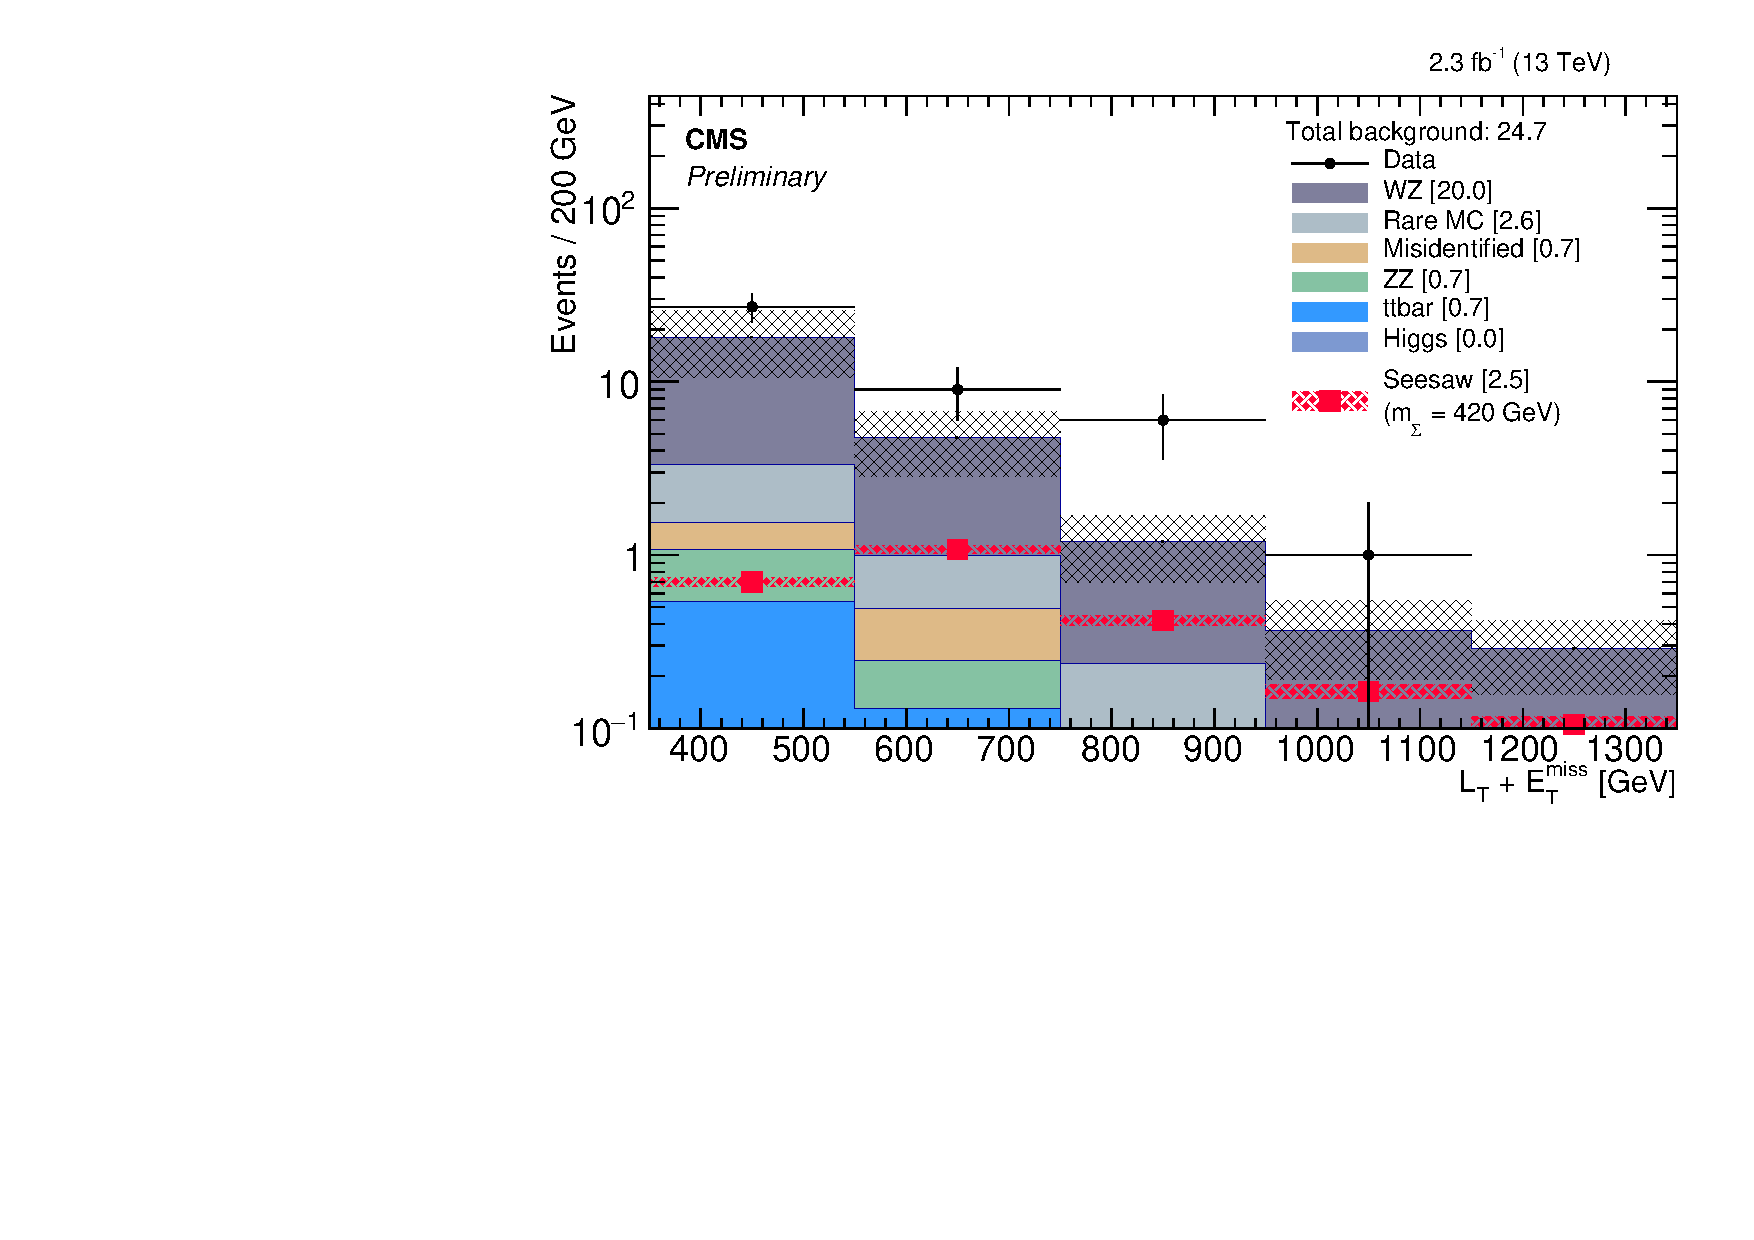
\includegraphics[width=\textwidth]{Results/plots/L3DYz1}
		\caption{3 leptons with OSSF pair on-\Z} \label{fig:Results/a}
	\end{subfigure}%
	\begin{subfigure}[b]{.5\textwidth}
		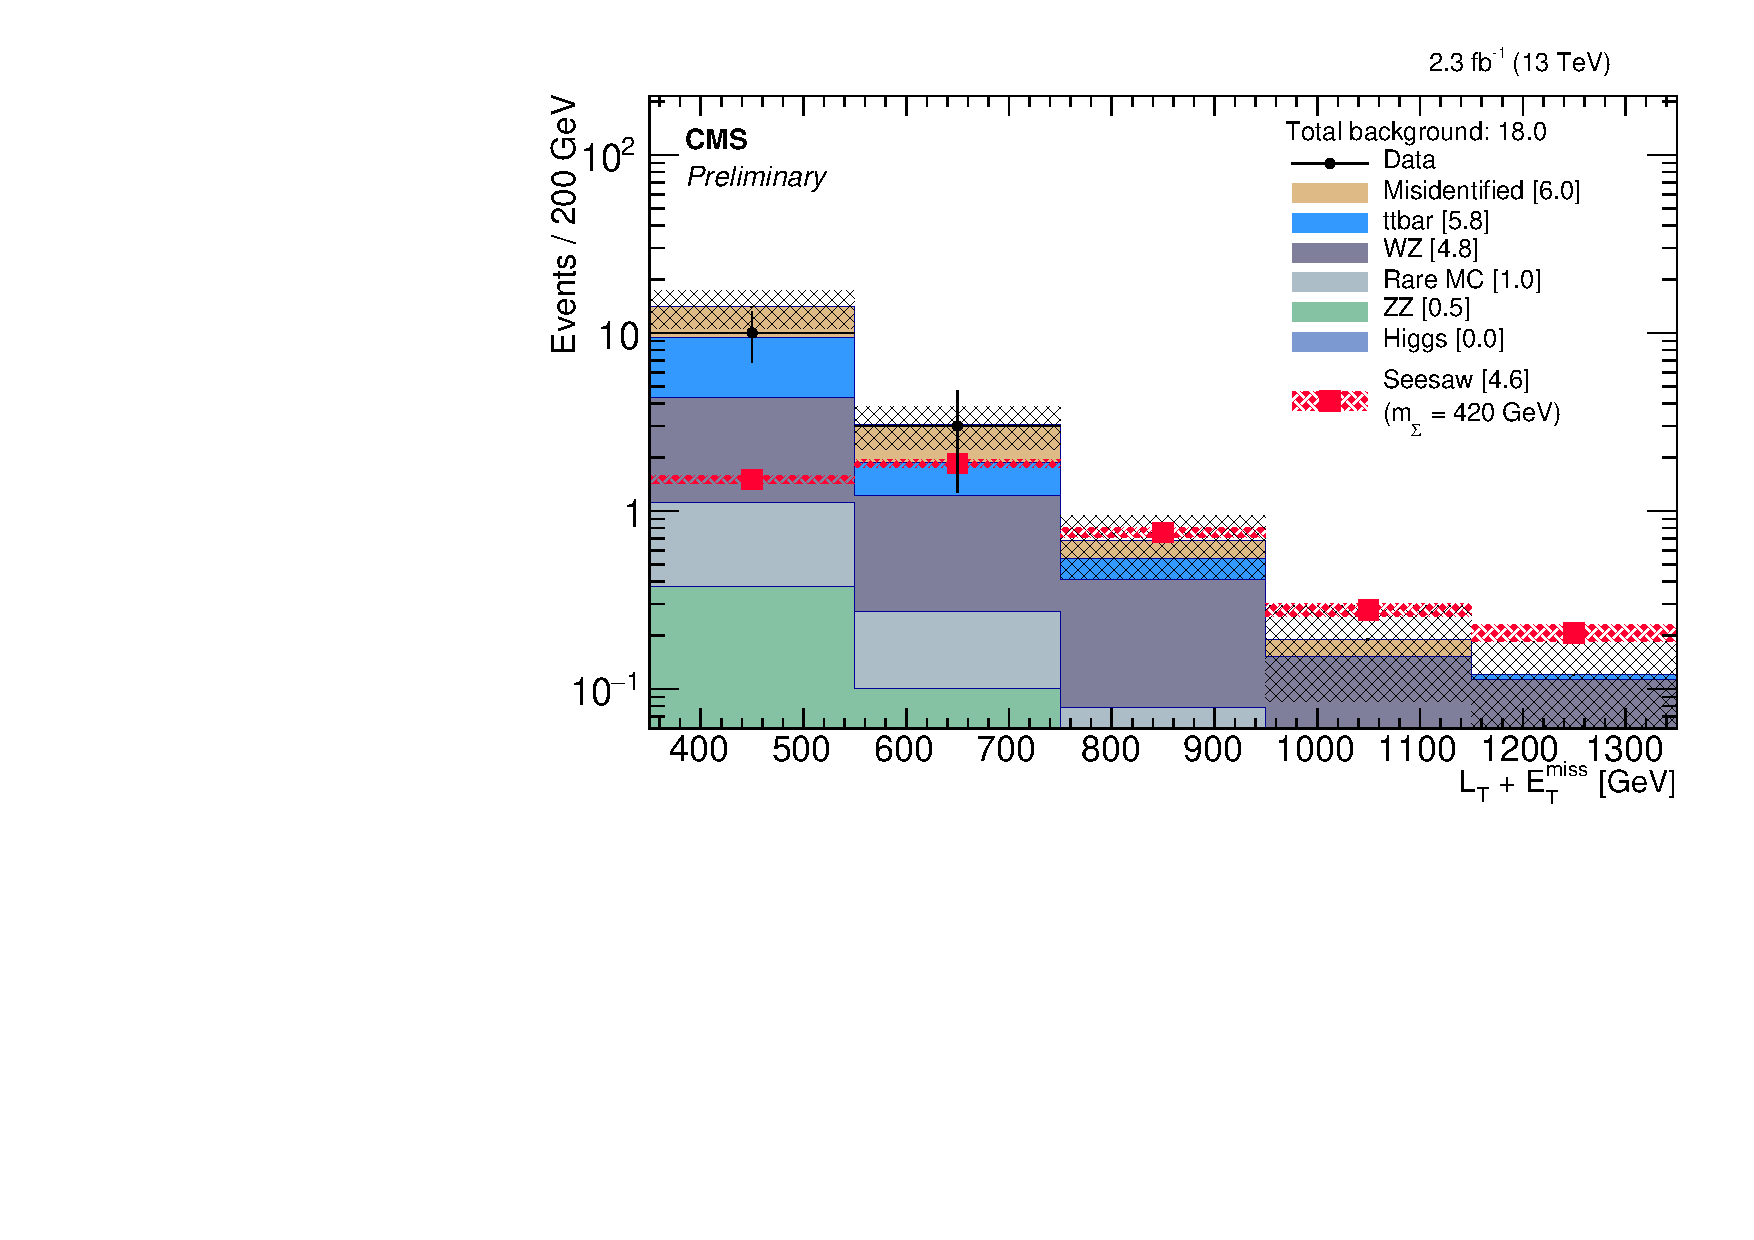
\includegraphics[width=\textwidth]{Results/plots/L3DYh1}
		\caption{3 leptons with OSSF pair above-\Z}
	\end{subfigure}
	\begin{subfigure}[b]{.5\textwidth}
		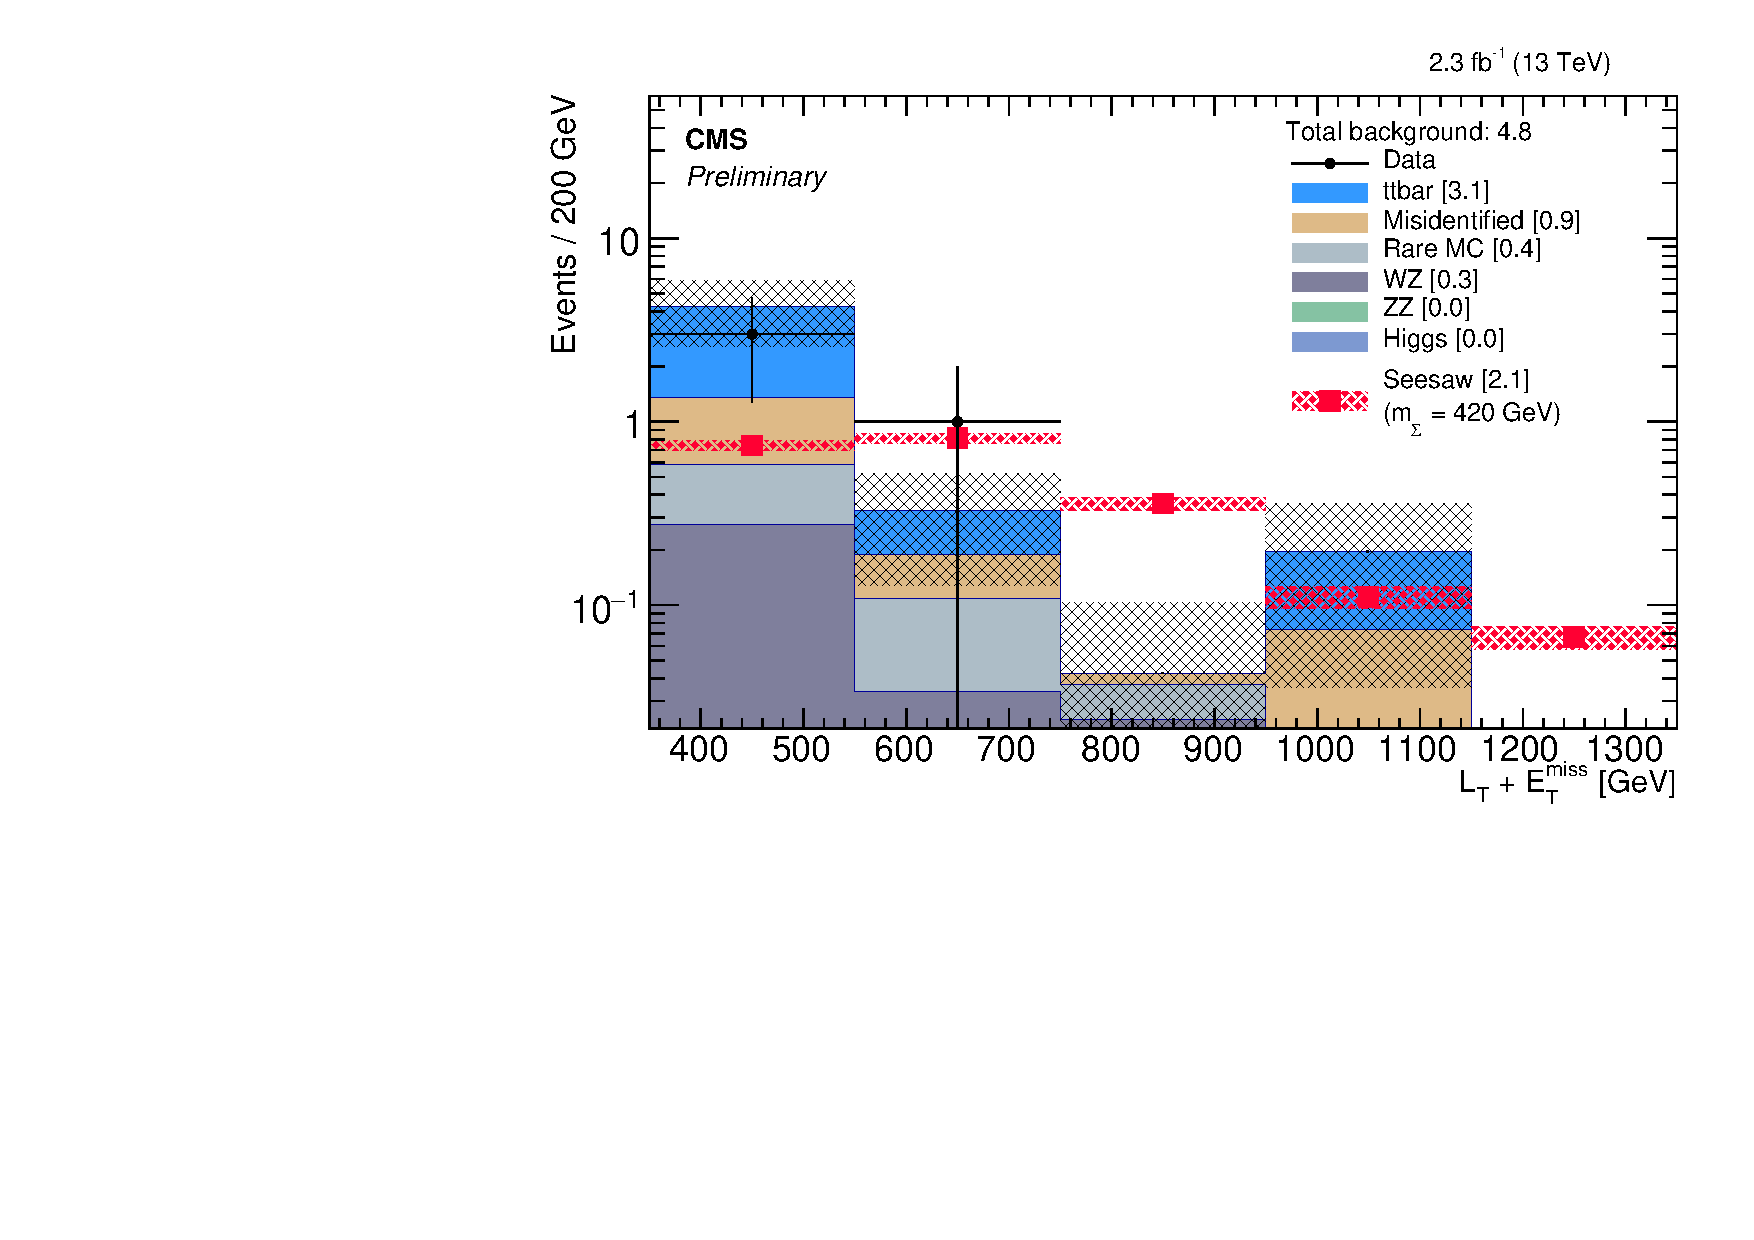
\includegraphics[width=\textwidth]{Results/plots/L3DY0}
		\caption{3 leptons, no OSSF pair}
	\end{subfigure}%
	\begin{subfigure}[b]{.5\textwidth}
		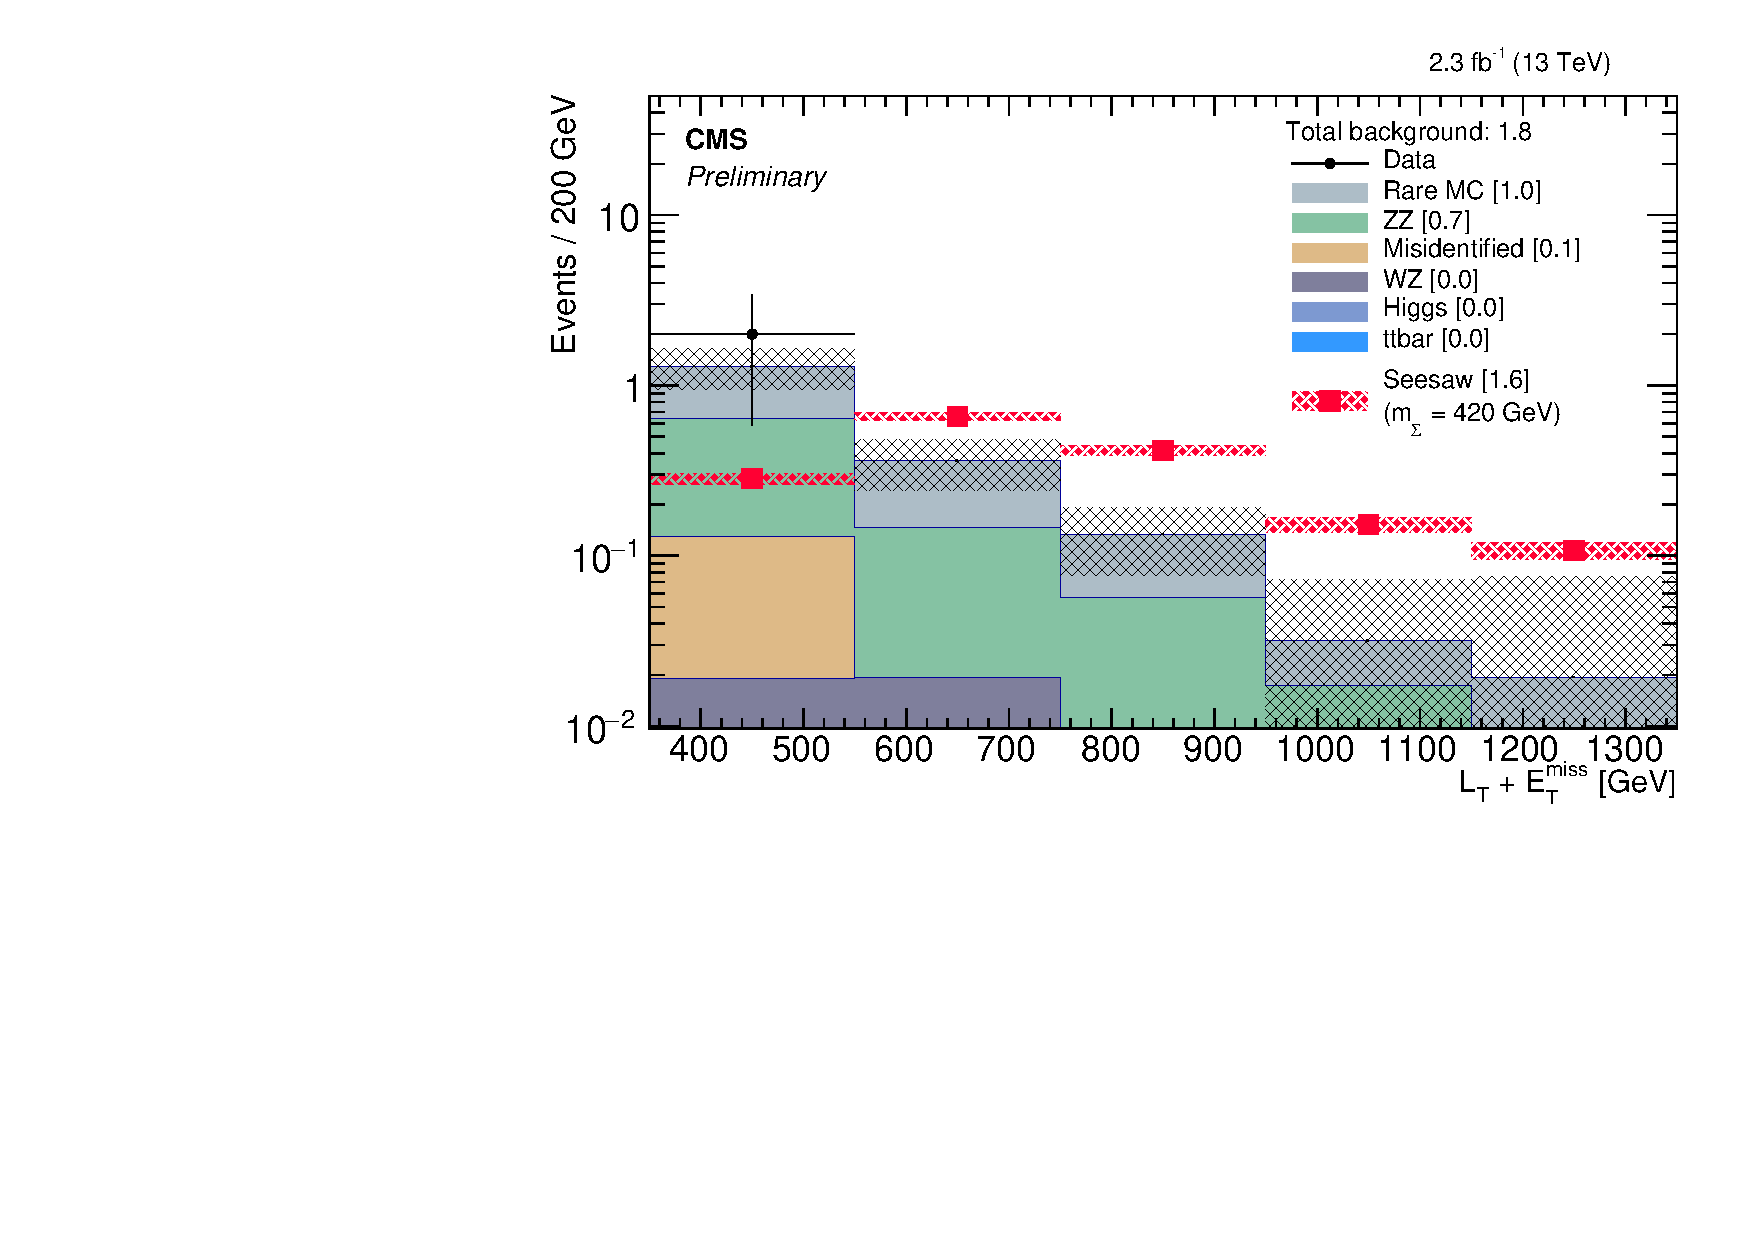
\includegraphics[width=\textwidth]{Results/plots/L4DYgt0}
		\caption{4 leptons, at least 1 OSSF pair}
	\end{subfigure}%
	\caption{Results: $L_\textrm{T} + \MET$ distributions (last bin includes overflow in all plots).
	\label{fig:Results}}
\end{center}
\end{sidewaysfigure}

The observations are generally consistent with the SM expectations, with the possible exception of the 3-lepton category that includes an OSSF lepton pair with invariant mass consistent with that of the Z boson (Fig.~\ref{fig:Results/a}). The dominant background for this category is the \WZ diboson production, as shown. The $p$-value for the observation in the aggregated twenty $L_\textrm{T} + \MET$ bins for the four categories shown in Fig.~\ref{fig:Results}, assuming SM physics only, is 0.93. This overall consistency with the SM expectation conveys the message that the apparent excess of observed events in the Fig.~\ref{fig:Results/a} is either a statistical artifact or a discrepancy that can be addressed only with additional data.

\section{Interpretation for the Seesaw Model}
\label{sec:Interpretation}
\label{sec:Interpretation/Seesaw}

As no statistically significant excess was observed, we calculate expected and observed upper limits on the cross section sum for the production of seesaw heavy fermion pairs ($\Sigma^0\Sigma^+$, $\Sigma^0\Sigma^-$, or $\Sigma^+\Sigma^-$), assuming a flavor-democratic value for the mixing angle parameters, $V_e = V_\mu = V_\tau = 10^{-6}$, and degenerate heavy fermion masses $m_\Sigma$.
By comparing with the signal production cross section, one can translate the cross section limits into limits on the heavy fermion mass which can be excluded based on the data.
The calculation is done using asymptotic CL$_s$ limits with a confidence level of 95\,\% \cite{Junk:1999kv,Read:2000ru,Read:2002hq}.
%Taking the ratio of the cross section upper limit and the signal cross section, one obtains the so-called $r$-value which indicates whether the signal at hand is excluded ($r < 1$) or cannot be excluded ($r > 1$).

Fig.~\ref{fig:exclusions} shows the mass limits for each of the categories presented in Fig.~\ref{fig:Results}. It can be seen that the observed limit is better, i.\,e. lower, than the expected limit whenever there is a deficiency observed in data. Similary, when the data is high, the observed limit is worse than expected. This is the case in particular for the observed limit in Fig.~\ref{fig:exclusions/a}, as there is an excess of events in the corresponding signal region (Fig.~\ref{fig:Results/a}). However, the impact of this excess on the overall result is limited, as this particular signal region is not very sensitive to the type-III seesaw signal and thus yields cross section limits that are much higher than those of the other signal regions limits (see Appendix~\ref{app:RelativeSensitivity}). This can also be seen by the fact that this signal region is the only one that is not sensitive enough to exclude any of the masses probed, while the other signal regions achieve mass limits between 300 and 380\,\GeV on their own. (Masses to the left of the intersection point are excluded.)

\begin{sidewaysfigure}
\begin{center}
	\begin{subfigure}[b]{.5\textwidth}
		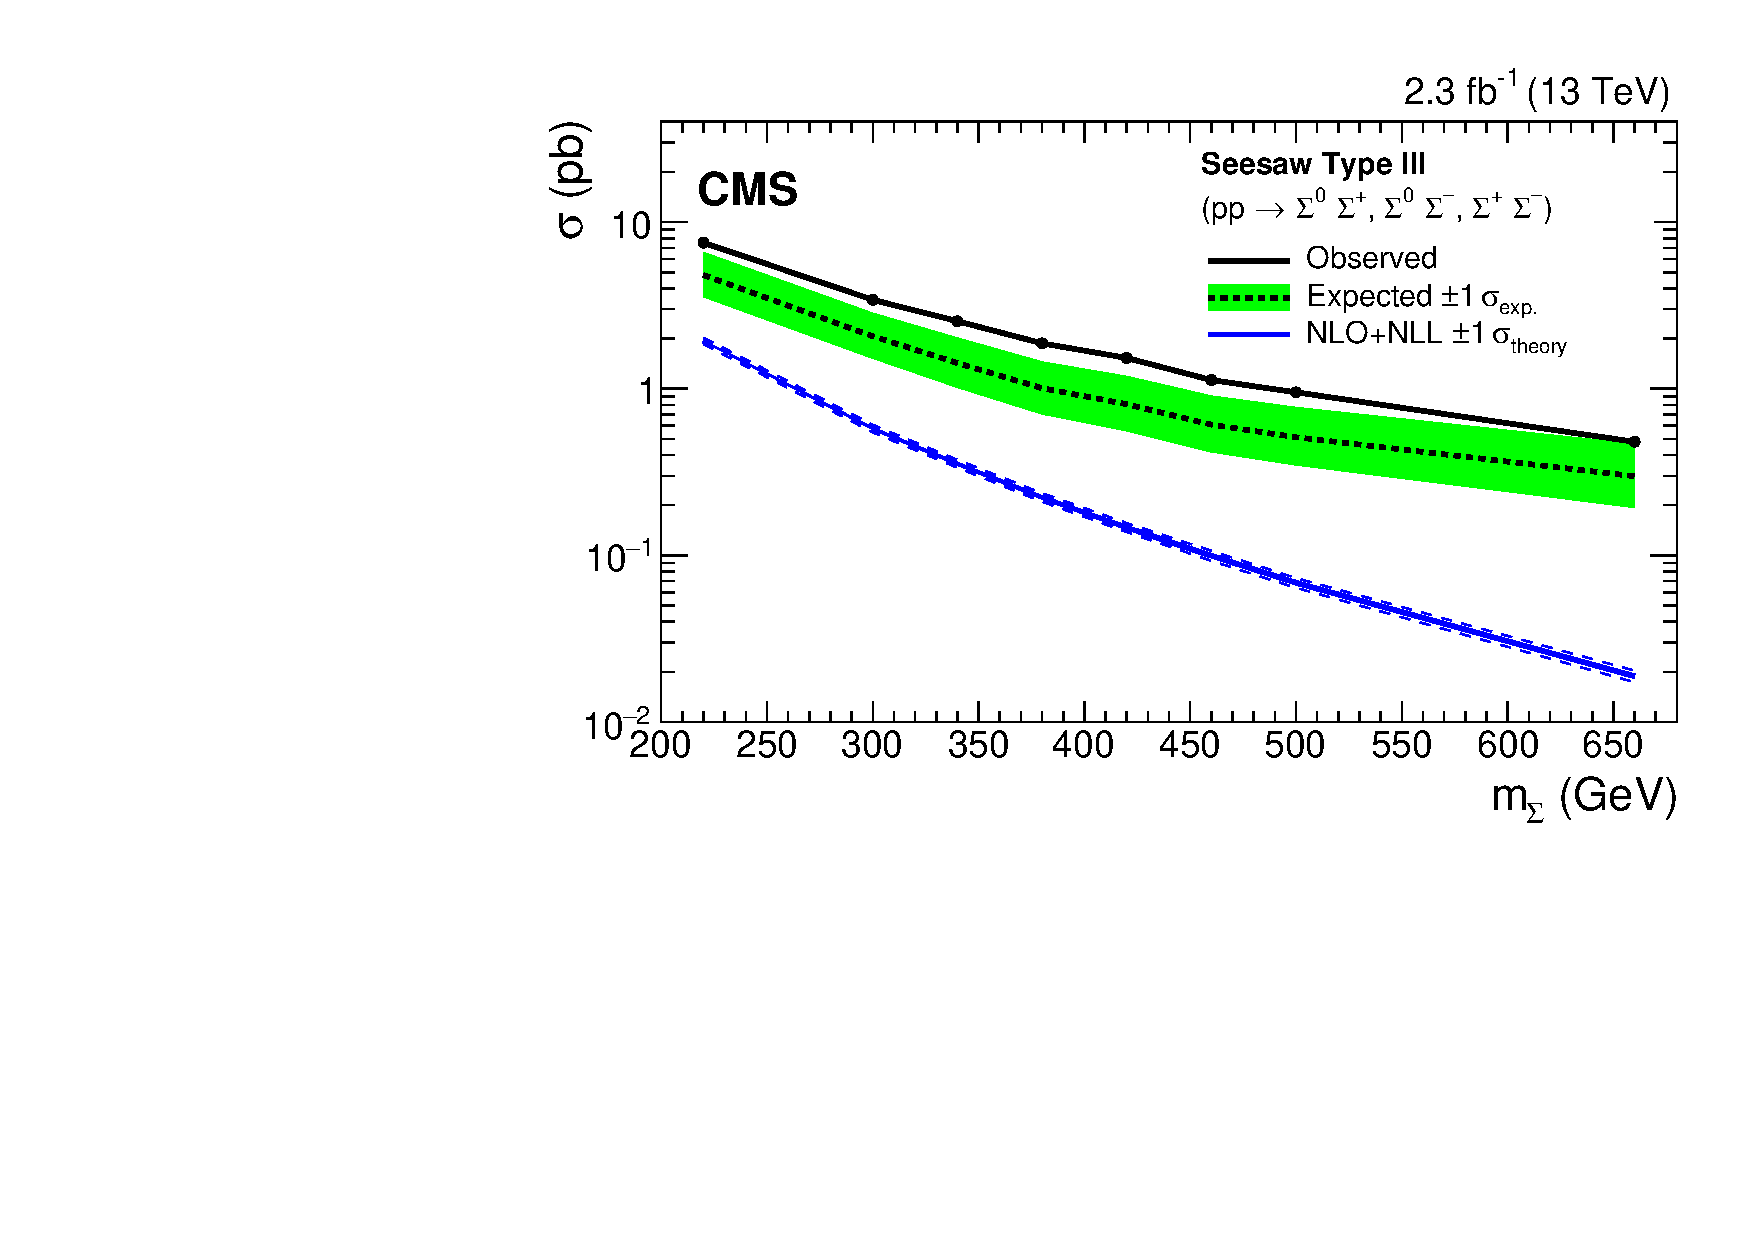
\includegraphics[width=\textwidth]{Results/exclusion-L3DYz1}
		\caption{3 leptons with OSSF pair on-\Z} \label{fig:exclusions/a}
	\end{subfigure}%
	\begin{subfigure}[b]{.5\textwidth}
		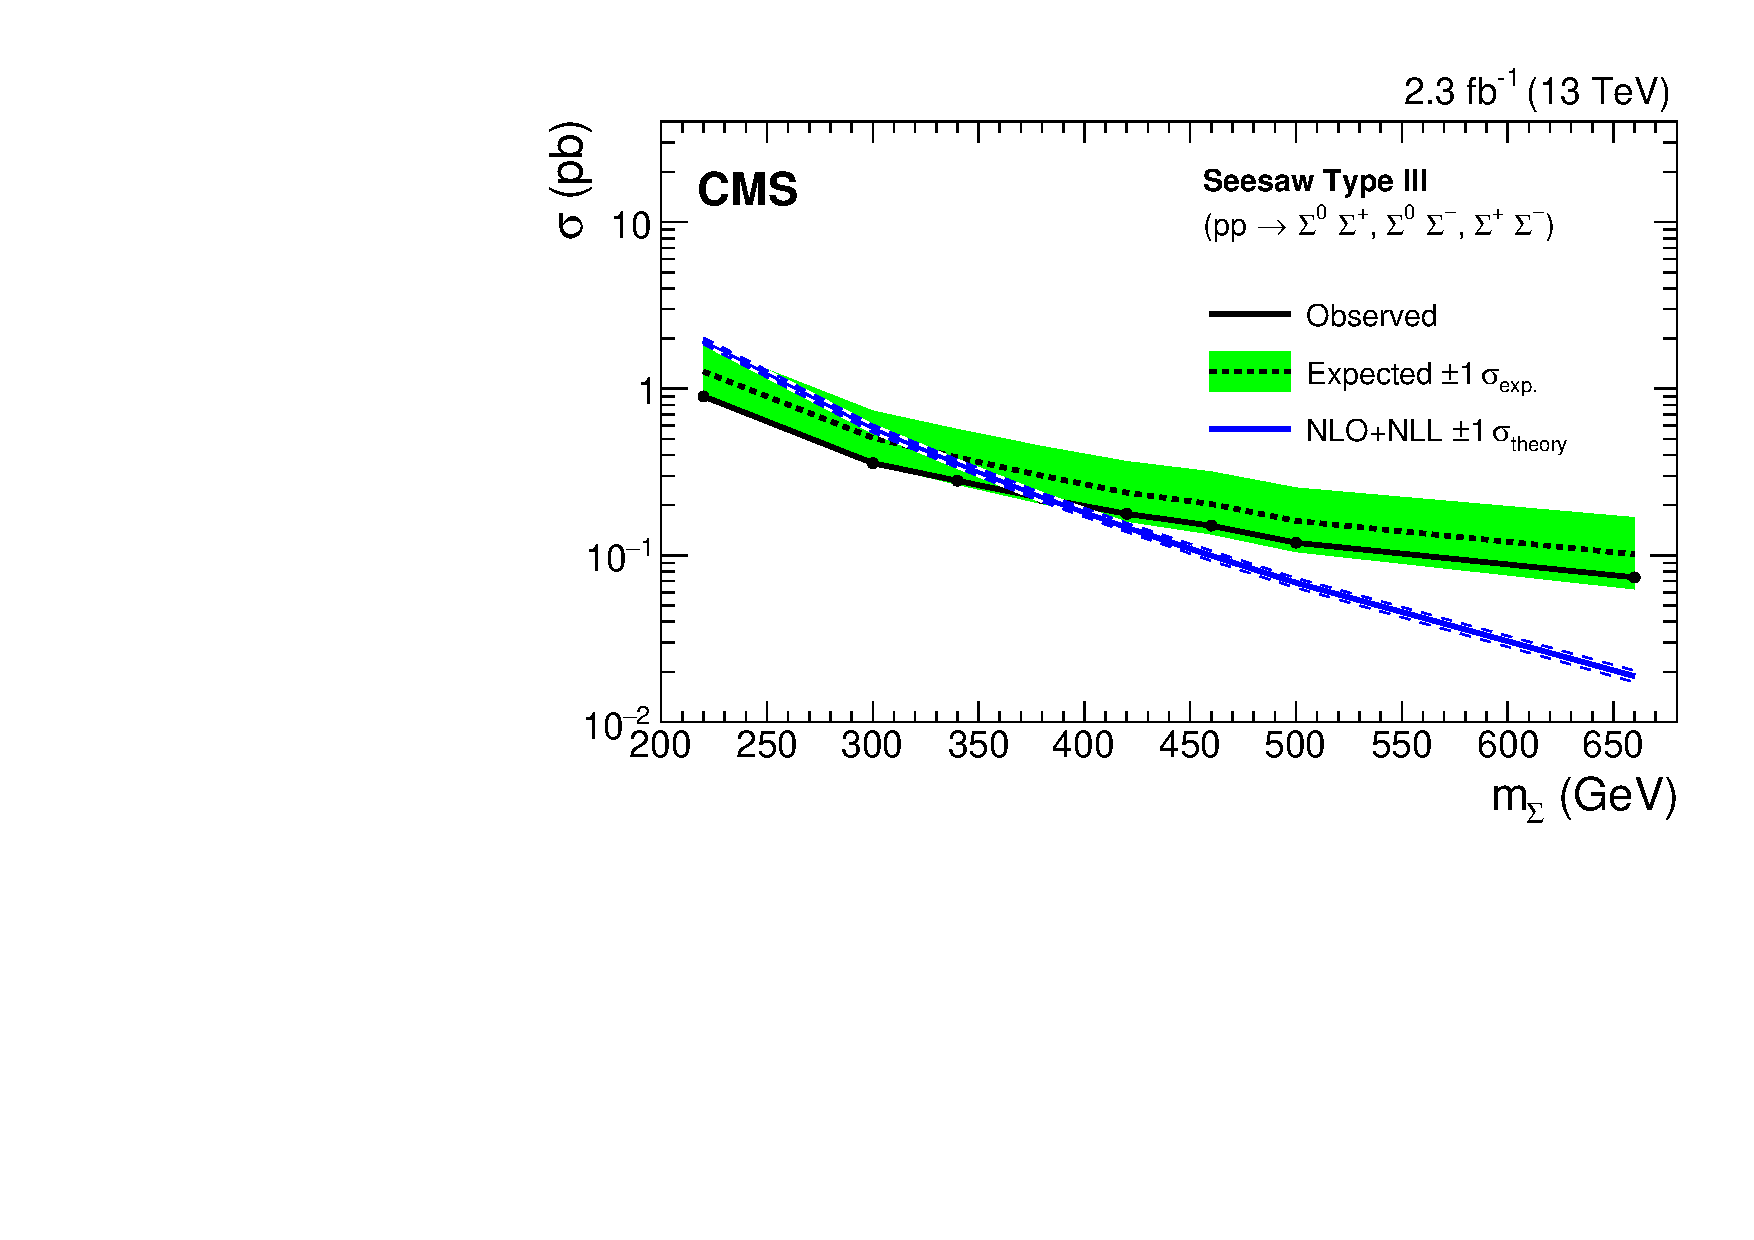
\includegraphics[width=\textwidth]{Results/exclusion-L3DYh1}
		\caption{3 leptons with OSSF pair above-\Z}
	\end{subfigure}
	\begin{subfigure}[b]{.5\textwidth}
		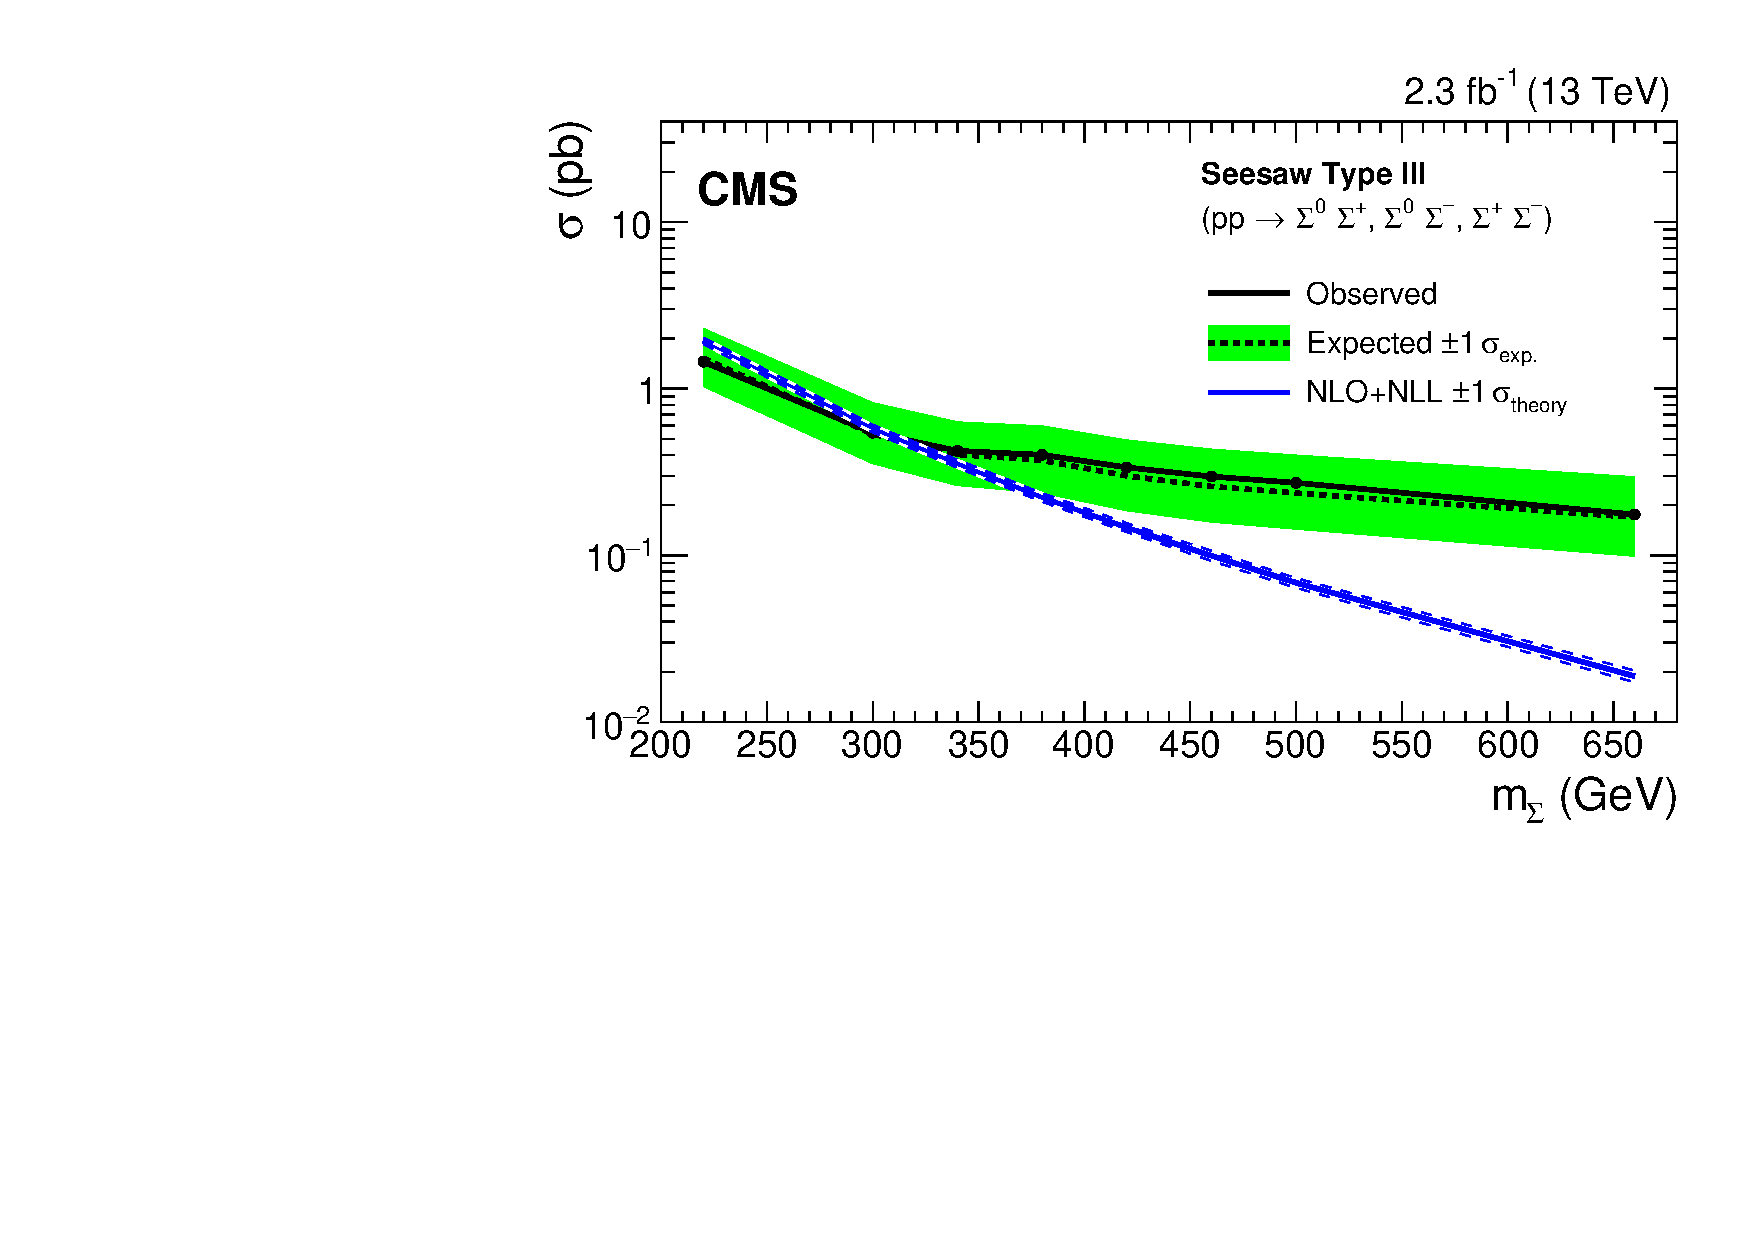
\includegraphics[width=\textwidth]{Results/exclusion-L3DY0}
		\caption{3 leptons, no OSSF pair}
	\end{subfigure}%
	\begin{subfigure}[b]{.5\textwidth}
		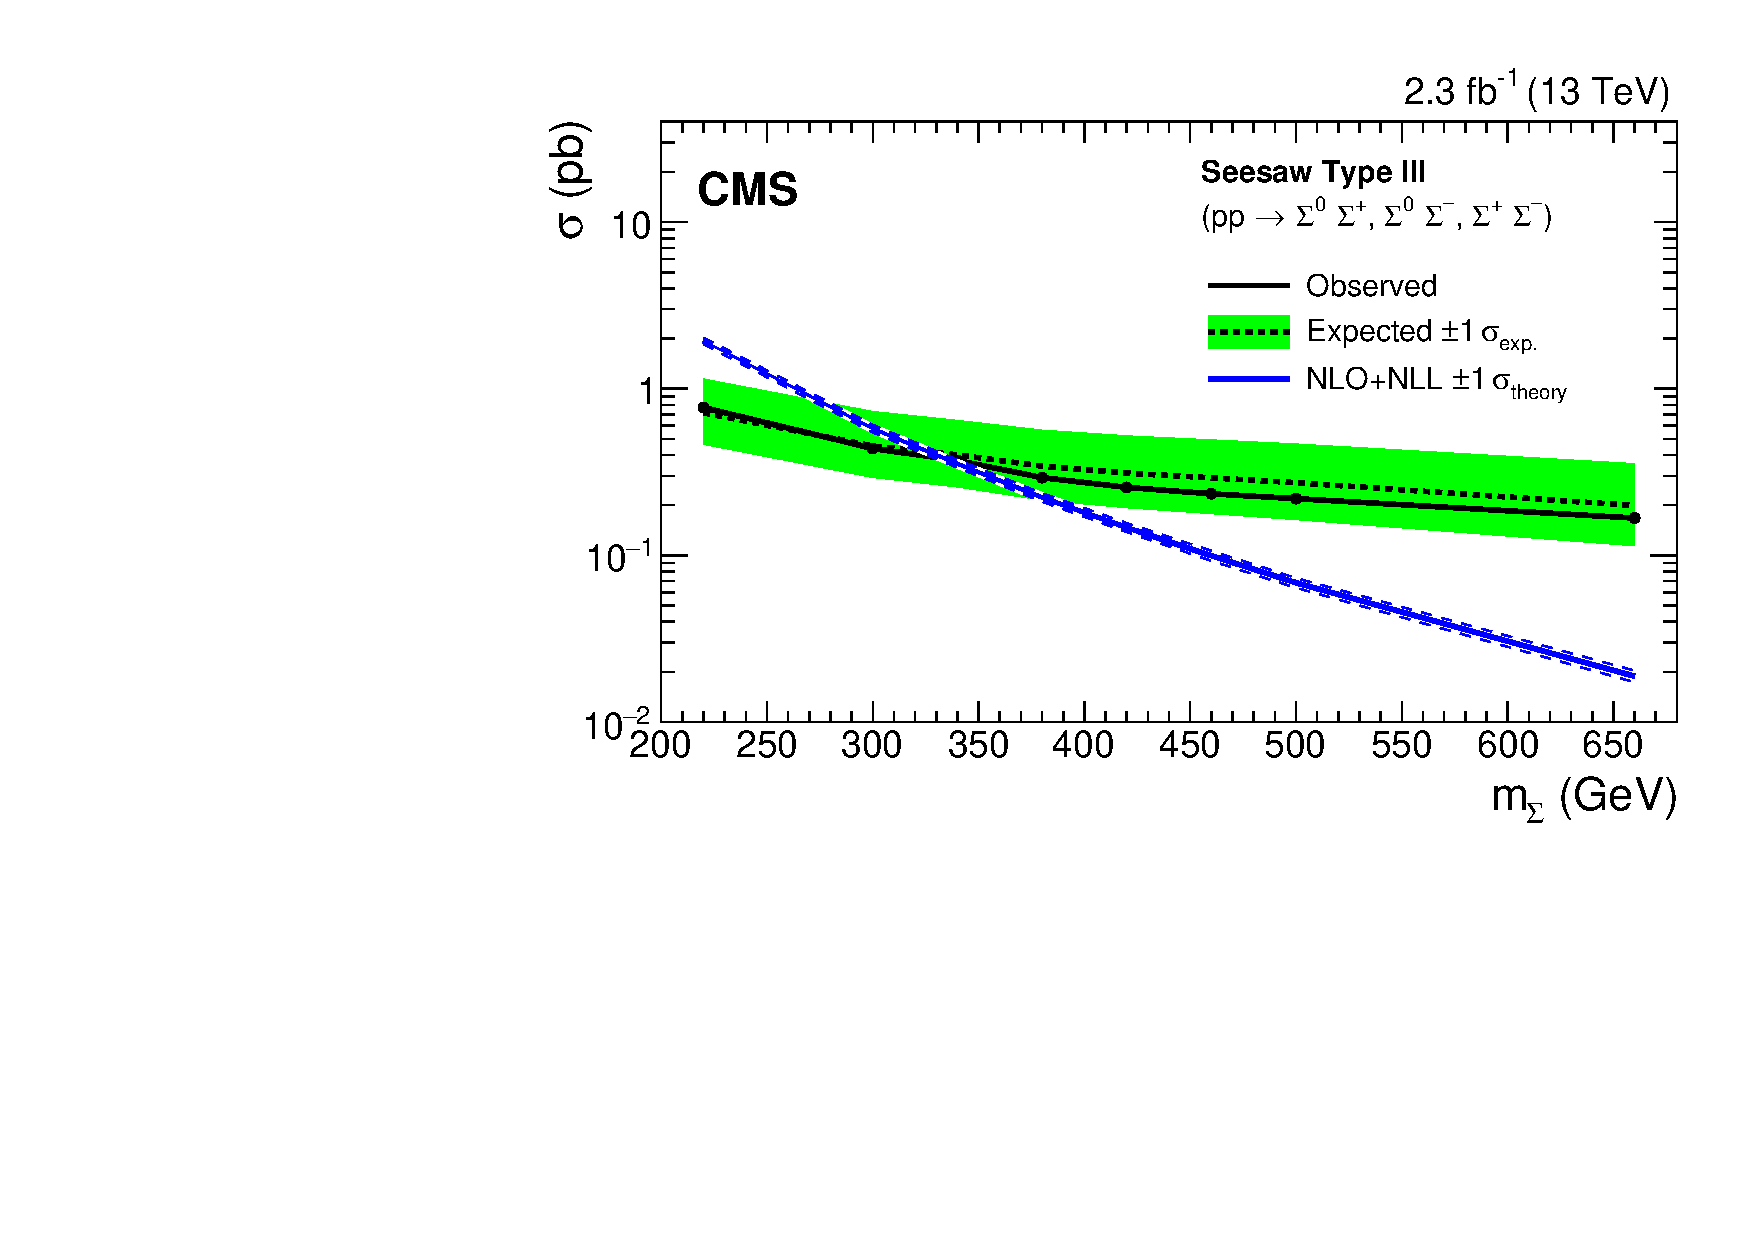
\includegraphics[width=\textwidth]{Results/exclusion-L4DYgt0}
		\caption{4 leptons, at least 1 OSSF pair}
	\end{subfigure}%
	\caption{Results: Exclusion curves. Masses to the left of the intersection point are excluded.
	\label{fig:exclusions}}
\end{center}
\end{sidewaysfigure}

If the data agreed perfectly with the background estimates in all signal regions combined, we would expect our analysis to exclude type-III seesaw heavy fermion pair production for masses below $m_\Sigma = 430\,\GeV$. The combined observed limit is at 440\,\GeV. The full exclusion curve is shown in Fig.~\ref{fig:exclusion}.

\begin{figure}[t]
\begin{center}
	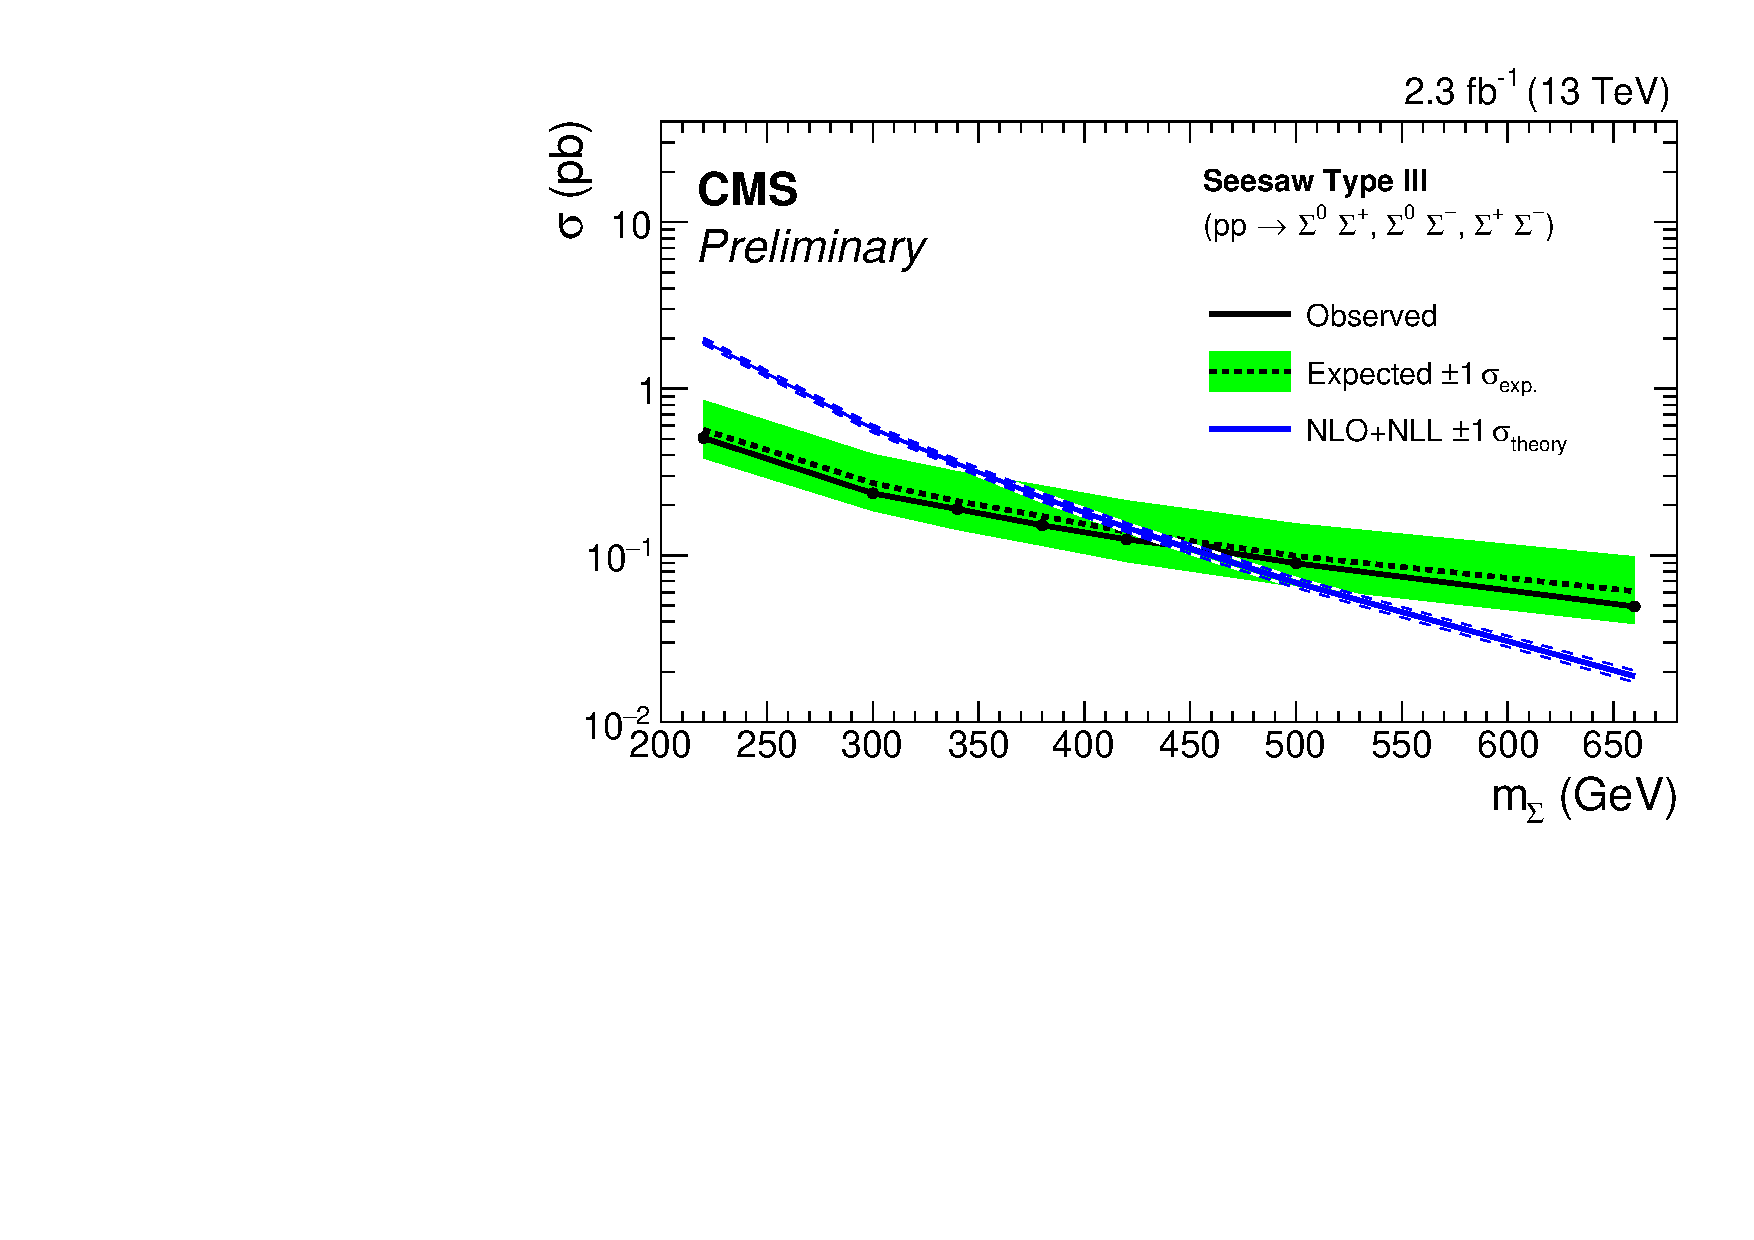
\includegraphics[width=.8\textwidth]{Results/exclusion}
	\caption{Exclusion for the flavor-democratic type-III seesaw model ($V_e = V_\mu = V_\tau = 10^{-6}$). We exclude heavy fermion pair production for masses below $m_\Sigma = 440\,\GeV$ (expected: 430\,\GeV) and give upper limits on the pair production cross section.
	\label{fig:exclusion}}
\end{center}
\end{figure}

In comparison to the Run-I results, the search sensitivity has been enhanced by various improvements, most notably the inclusion of new decay modes involving the Higgs boson and of 4-lepton channels, as well as by the introduction of an improved fine-grained binning scheme. Exclusion limits from the CMS Run I result were at $m_\Sigma = 250\,\GeV$ (expected) and $m_\Sigma = 278\,\GeV$ (observed) \cite{CMS-PAS-EXO-14-001}.
